\documentclass[a4paper, 12pt]{article}

\newcommand{\languages}{french, english}

%%%%% Tools

\usepackage{comment}
\usepackage{lipsum}
\usepackage{xstring}

%%%%% Document

\usepackage[pdfusetitle]{hyperref}

\usepackage{geometry}
\geometry{paper=a4paper,top=3.5cm,bottom=2.5cm,right=2.5cm,left=2.5cm}

\usepackage{fancyhdr}
\pagestyle{fancy}
\fancyhead[L]{}
\fancyhead[R]{\leftmark}
\fancyfoot[C]{\thepage}
\renewcommand{\headrulewidth}{0pt}

%%%%% Text

\usepackage[utf8]{inputenc}
\usepackage[T1]{fontenc}
\usepackage[parfill]{parskip}
\usepackage{csquotes}

\newlength{\mytextsize}
\makeatletter
\setlength{\mytextsize}{\f@size pt}
\makeatother

%%%%% Languages

\ifx\languages\undefined
	\usepackage[english, french]{babel}
\else
	\usepackage[\languages]{babel}
\fi

% english

\addto\captionsenglish{\def\figurename{Figure}}
\addto\captionsenglish{\def\tablename{Table}}

\newcommand{\st}{\text{s.t.}}

\IfStrEq{\languagename}{english}{
	\newcommand{\lgpreamble}{Preamble}
}

% french

\frenchbsetup{StandardLists=true}

\addto\captionsfrench{\def\figurename{Figure}}
\addto\captionsfrench{\def\tablename{Table}}
\addto\captionsfrench{\def\proofname{Preuve}}

\newcommand{\tq}{\text{t.q.}}
\newcommand{\cad}{c.-à-d. }
\newcommand{\Cad}{C.-à-d. }

\IfStrEq{\languagename}{french}{
	\newcommand{\lgpreamble}{Préambule}
}

%%%%% Styles

\usepackage[skip=\mytextsize]{caption}
\usepackage{float}
\usepackage{mdframed}
\usepackage{enumitem}
\usepackage{eurosym}
\usepackage{color}

\newcommand\caaption[1]{\caption{#1}\vspace{-1\mytextsize}}

%%%%% Mathematics

\usepackage{amsmath}
\usepackage{amssymb}
\usepackage{amsfonts}
\usepackage{bm}
\usepackage{esint}
\usepackage[makeroom]{cancel}

\newcommand{\fact}[1]{#1!}
\newcommand{\e}[1]{\mathbf{e}_{#1}}
\newcommand{\deriv}{\mathrm{d}}
\DeclareMathOperator{\tr}{tr}


%%%%% SI units

\usepackage[squaren,Gray,cdot]{SIunits}
\usepackage{sistyle}

\IfStrEq{\languagename}{french}{
	\SIdecimalsign{,}
}

%%%%% Chemistry

\usepackage[version=4]{mhchem}

%%%%% Table & Figure

\usepackage{array}
\usepackage{tabularx}
\usepackage{multirow}
\usepackage{multicol}
\newcolumntype{M}[1]{>{\centering\arraybackslash}m{#1}}
%\setlength\extrarowheight{0em}
\renewcommand{\arraystretch}{1.3}

\usepackage{wrapfig}
\usepackage{pgfplots}
\usepackage{tikz}
\usetikzlibrary{shapes.geometric, positioning}
\usepackage{graphics}
\usepackage{graphicx}
\pgfplotsset{axis on top, compat = 1.3}

%%%%%% Theorems and Definitions

\usepackage{amsthm}
\usepackage{thmtools}

\IfStrEq{\languagename}{english}{
	\newcommand{\lgthm}{Theorem}
	\newcommand{\lglem}{Lemma}
	\newcommand{\lgprop}{Proposition}
	\newcommand{\lgdefn}{Definition}
	\newcommand{\lghyp}{Hypothesis}
	\newcommand{\lgquest}{Question}
	\newcommand{\lgansw}{Answer}
	\newcommand{\lgexpl}{Example}
	\newcommand{\lgrmk}{Remark}
	\newcommand{\lgnote}{Note}
	\newcommand{\lgtip}{Tip}
}

\IfStrEq{\languagename}{french}{
	\newcommand{\lgthm}{Théorème}
	\newcommand{\lglem}{Lemme}
	\newcommand{\lgprop}{Proposition}
	\newcommand{\lgdefn}{Définition}
	\newcommand{\lghyp}{Hypothèse}
	\newcommand{\lgquest}{Question}
	\newcommand{\lgansw}{Réponse}
	\newcommand{\lgexpl}{Exemple}
	\newcommand{\lgrmk}{Remarque}
	\newcommand{\lgnote}{Note}
	\newcommand{\lgtip}{Conseil}
}

\theoremstyle{plain}
\newtheorem{thm}{\lgthm}[section]
\newtheorem{lem}{\lglem}[section]
\newtheorem{prop}{\lgprop}[section]

\theoremstyle{definition}
\newtheorem{defn}{\lgdefn}[section]
\newtheorem{hyp}{\lghyp}[section]
\newtheorem{quest}{\lgquest}[]

\declaretheorem[
name=\lgansw,
qed={\lower-0.3ex\hbox{$\triangle$}},
within=quest
]{answ}

\declaretheorem[
name=\lgexpl,
qed={\lower-0.3ex\hbox{$\triangle$}},
within=section
]{expl}

\theoremstyle{remark}
\newtheorem*{rmk}{\lgrmk}
\newtheorem*{note}{\lgnote}
\newtheorem*{tip}{\lgtip}

\begingroup
\makeatletter
\@for\theoremstyle:=definition,remark,plain\do{%
	\expandafter\g@addto@macro\csname th@\theoremstyle\endcsname{%
		\addtolength\thm@preskip\parskip
	}%
}
\endgroup

%%%% Others

\renewcommand{\qedsymbol}{$\blacksquare$}

\newcommand{\mytableofcontents}{
	\newpage
	\pagenumbering{roman}
	\tableofcontents
	\newpage
	\pagenumbering{arabic}
}

%%%%%%%%%%%%%%%%%%%

%%%%%%%%%%%%%%%%%%%

\newgeometry{margin = 2.5cm}

%%%%%%%%%%%%%%%%%%% maketitle

\title{Results of project 2 -- part 2}
\author{\textsc{Rozet} François}
\date{}

%%%%%%%%%%%%%%%%%%%

\usepackage{makecell}
\renewcommand\cellgape{\Gape[4pt]}

%%%%%%%%%%%%%%%%%%%

\begin{document}
	\maketitle
	\begin{table}[h]
		\centering
		\begin{tabular}{|c|c|c|c|c|c|}
			\hline
			Mode \no & \makecell{Measured\\frequency $[\hertz]$} & \makecell{2 DOF\\model $[\hertz]$} & \makecell{Relative\\error $[\%]$} & \makecell{Rayleigh-Ritz\\method $[\hertz]$} & \makecell{Relative\\error $[\%]$} \\ \hline\hline
			   1     &               \num{8.8293}                &            \num{8.6962}            &            \num{-1.51}            &                \num{8.6615}                 &            \num{-1.90}            \\ \hline
			   2     &              \num{1.2281e1}               &           \num{1.2351e1}           &            \num{0.57}             &               \num{1.2292e1}                &            \num{0.08}             \\ \hline
			   3     &              \num{6.3681e1}               &                 --                 &                --                 &               \num{6.4170e1}                &            \num{0.77}             \\ \hline
			   4     &              \num{1.6098e2}               &                 --                 &                --                 &               \num{1.6055e2}                &            \num{-0.27}            \\ \hline
			   5     &              \num{3.2303e2}               &                 --                 &                --                 &               \num{3.2255e2}                &            \num{-0.15}             \\ \hline
		\end{tabular}
		\caaption{Frequencies}
		\label{table:frequencies}
	\end{table}
	\begin{figure}[h]
		\centering
		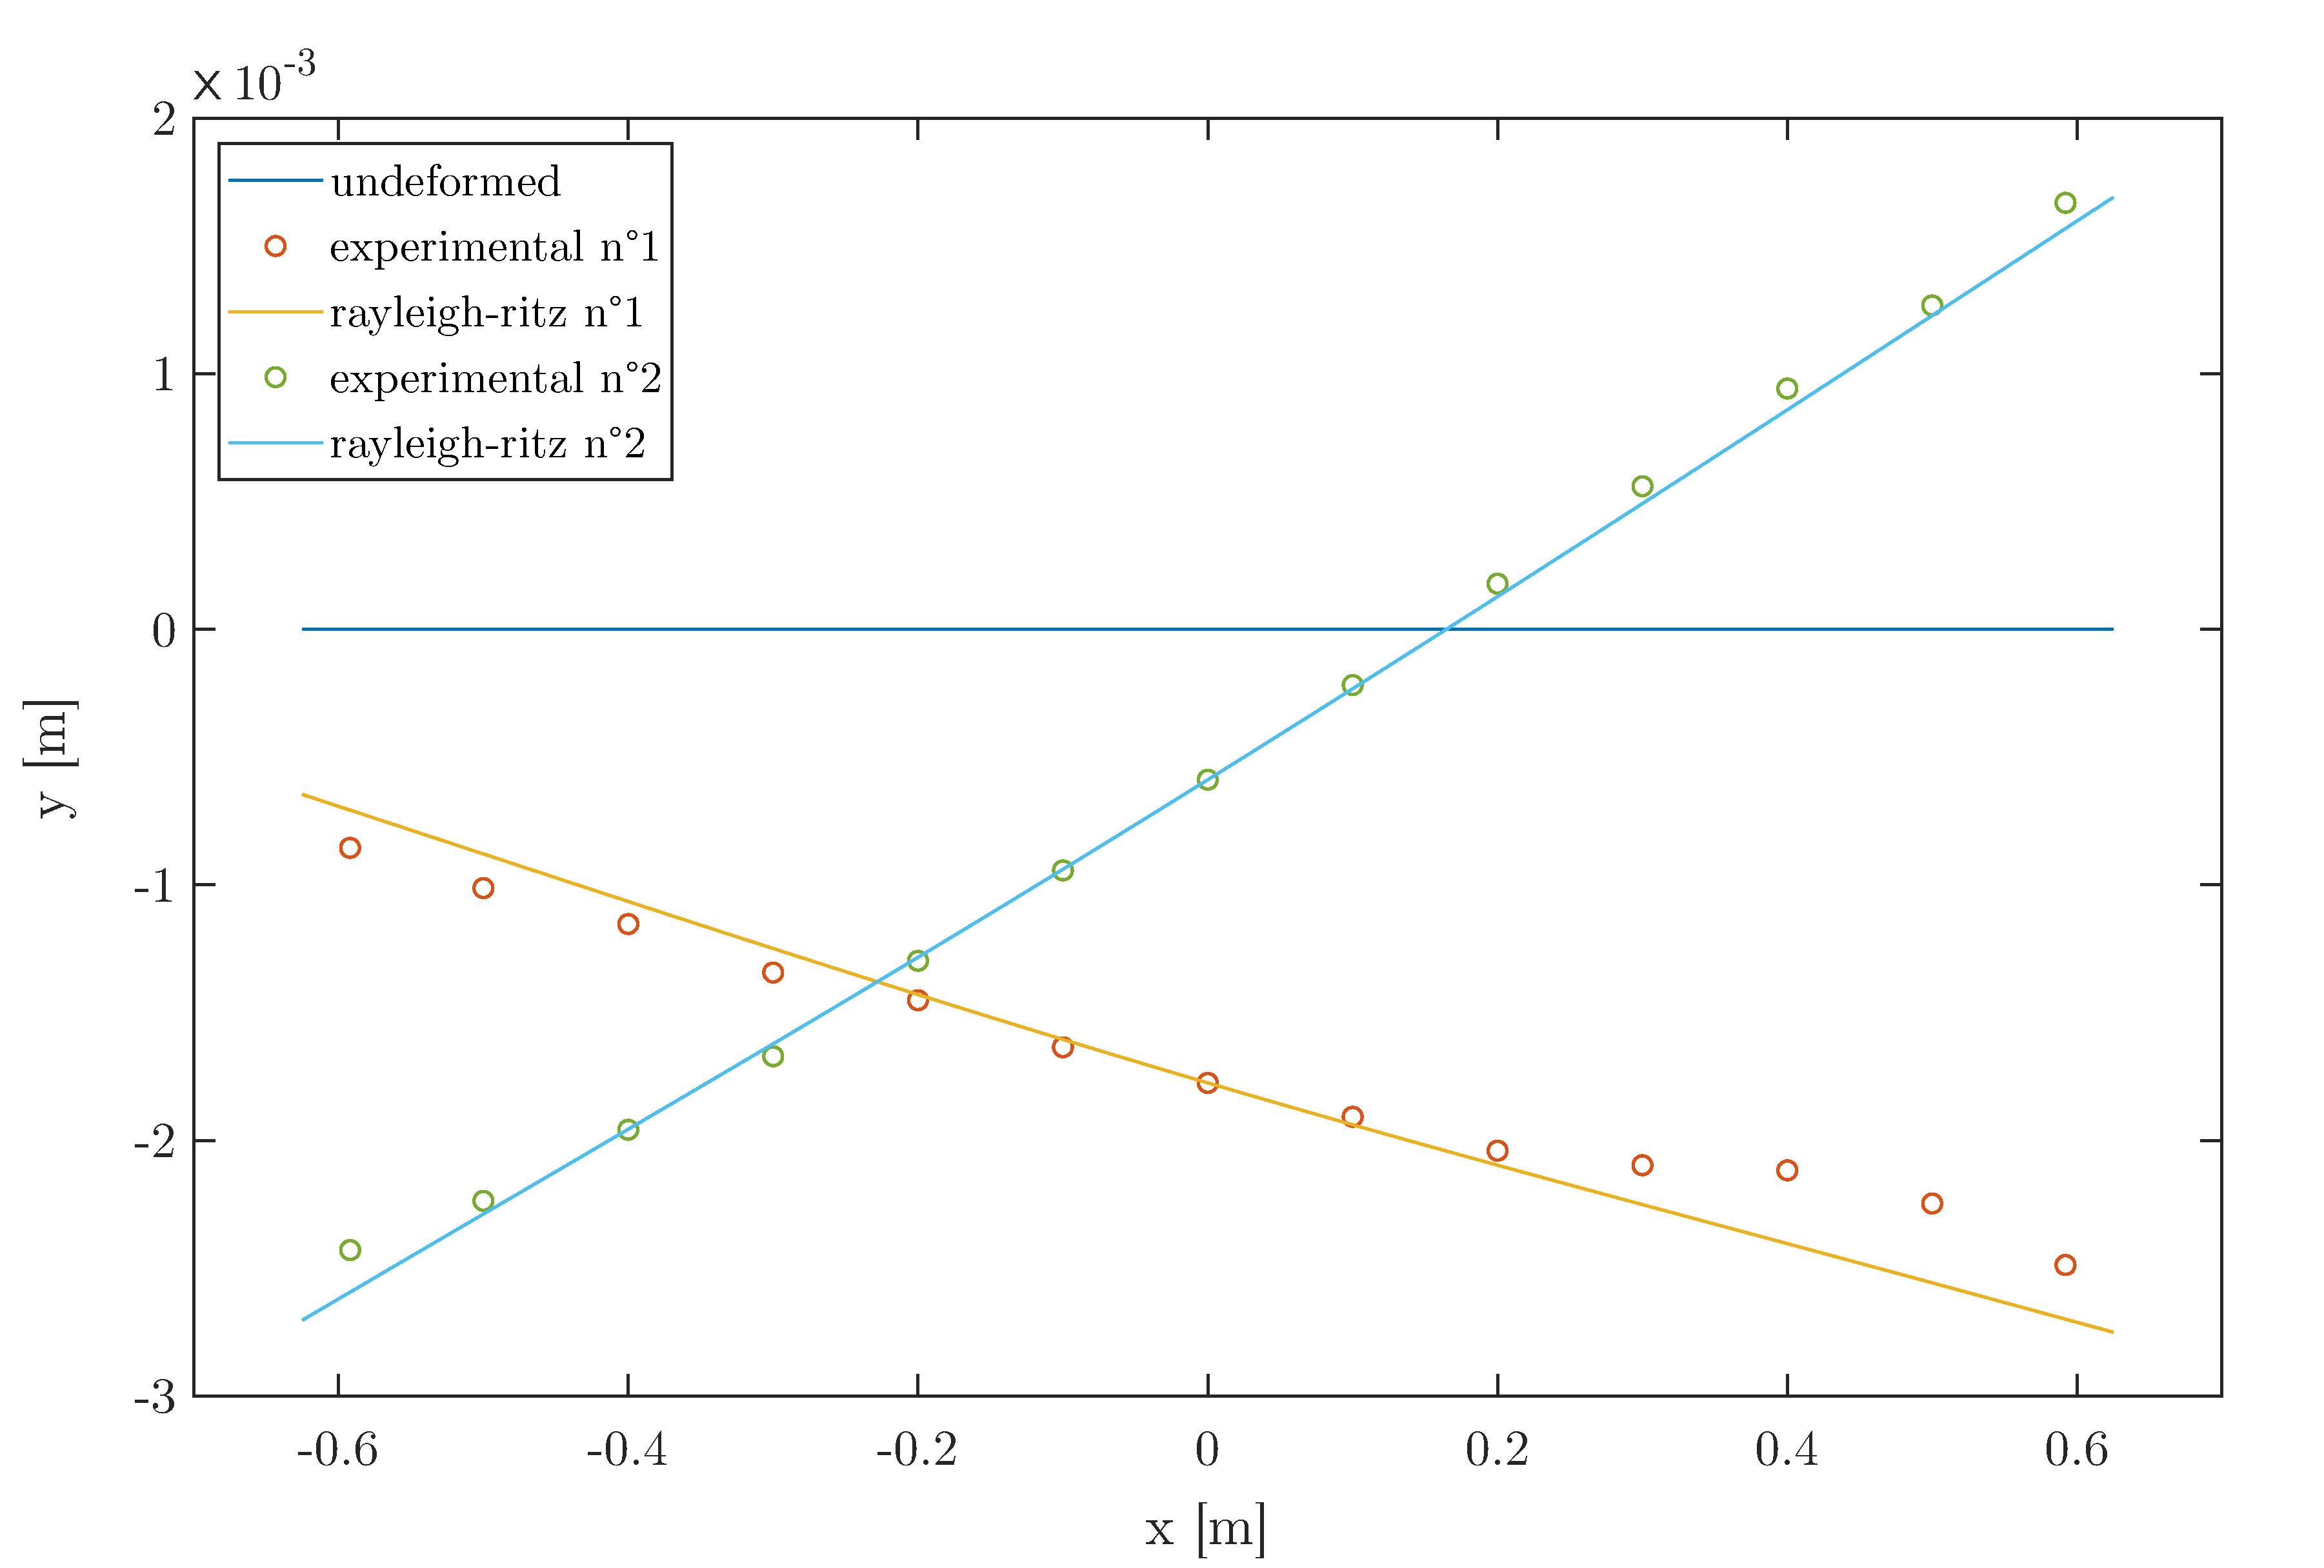
\includegraphics[width=1\textwidth]{resources/pdf/mode-shapes1and2.pdf}
		\caption{Mode-shapes \no 1 and 2}
		\label{figure:modeshape12}
	\end{figure}
	\begin{figure}[h]
		\centering
		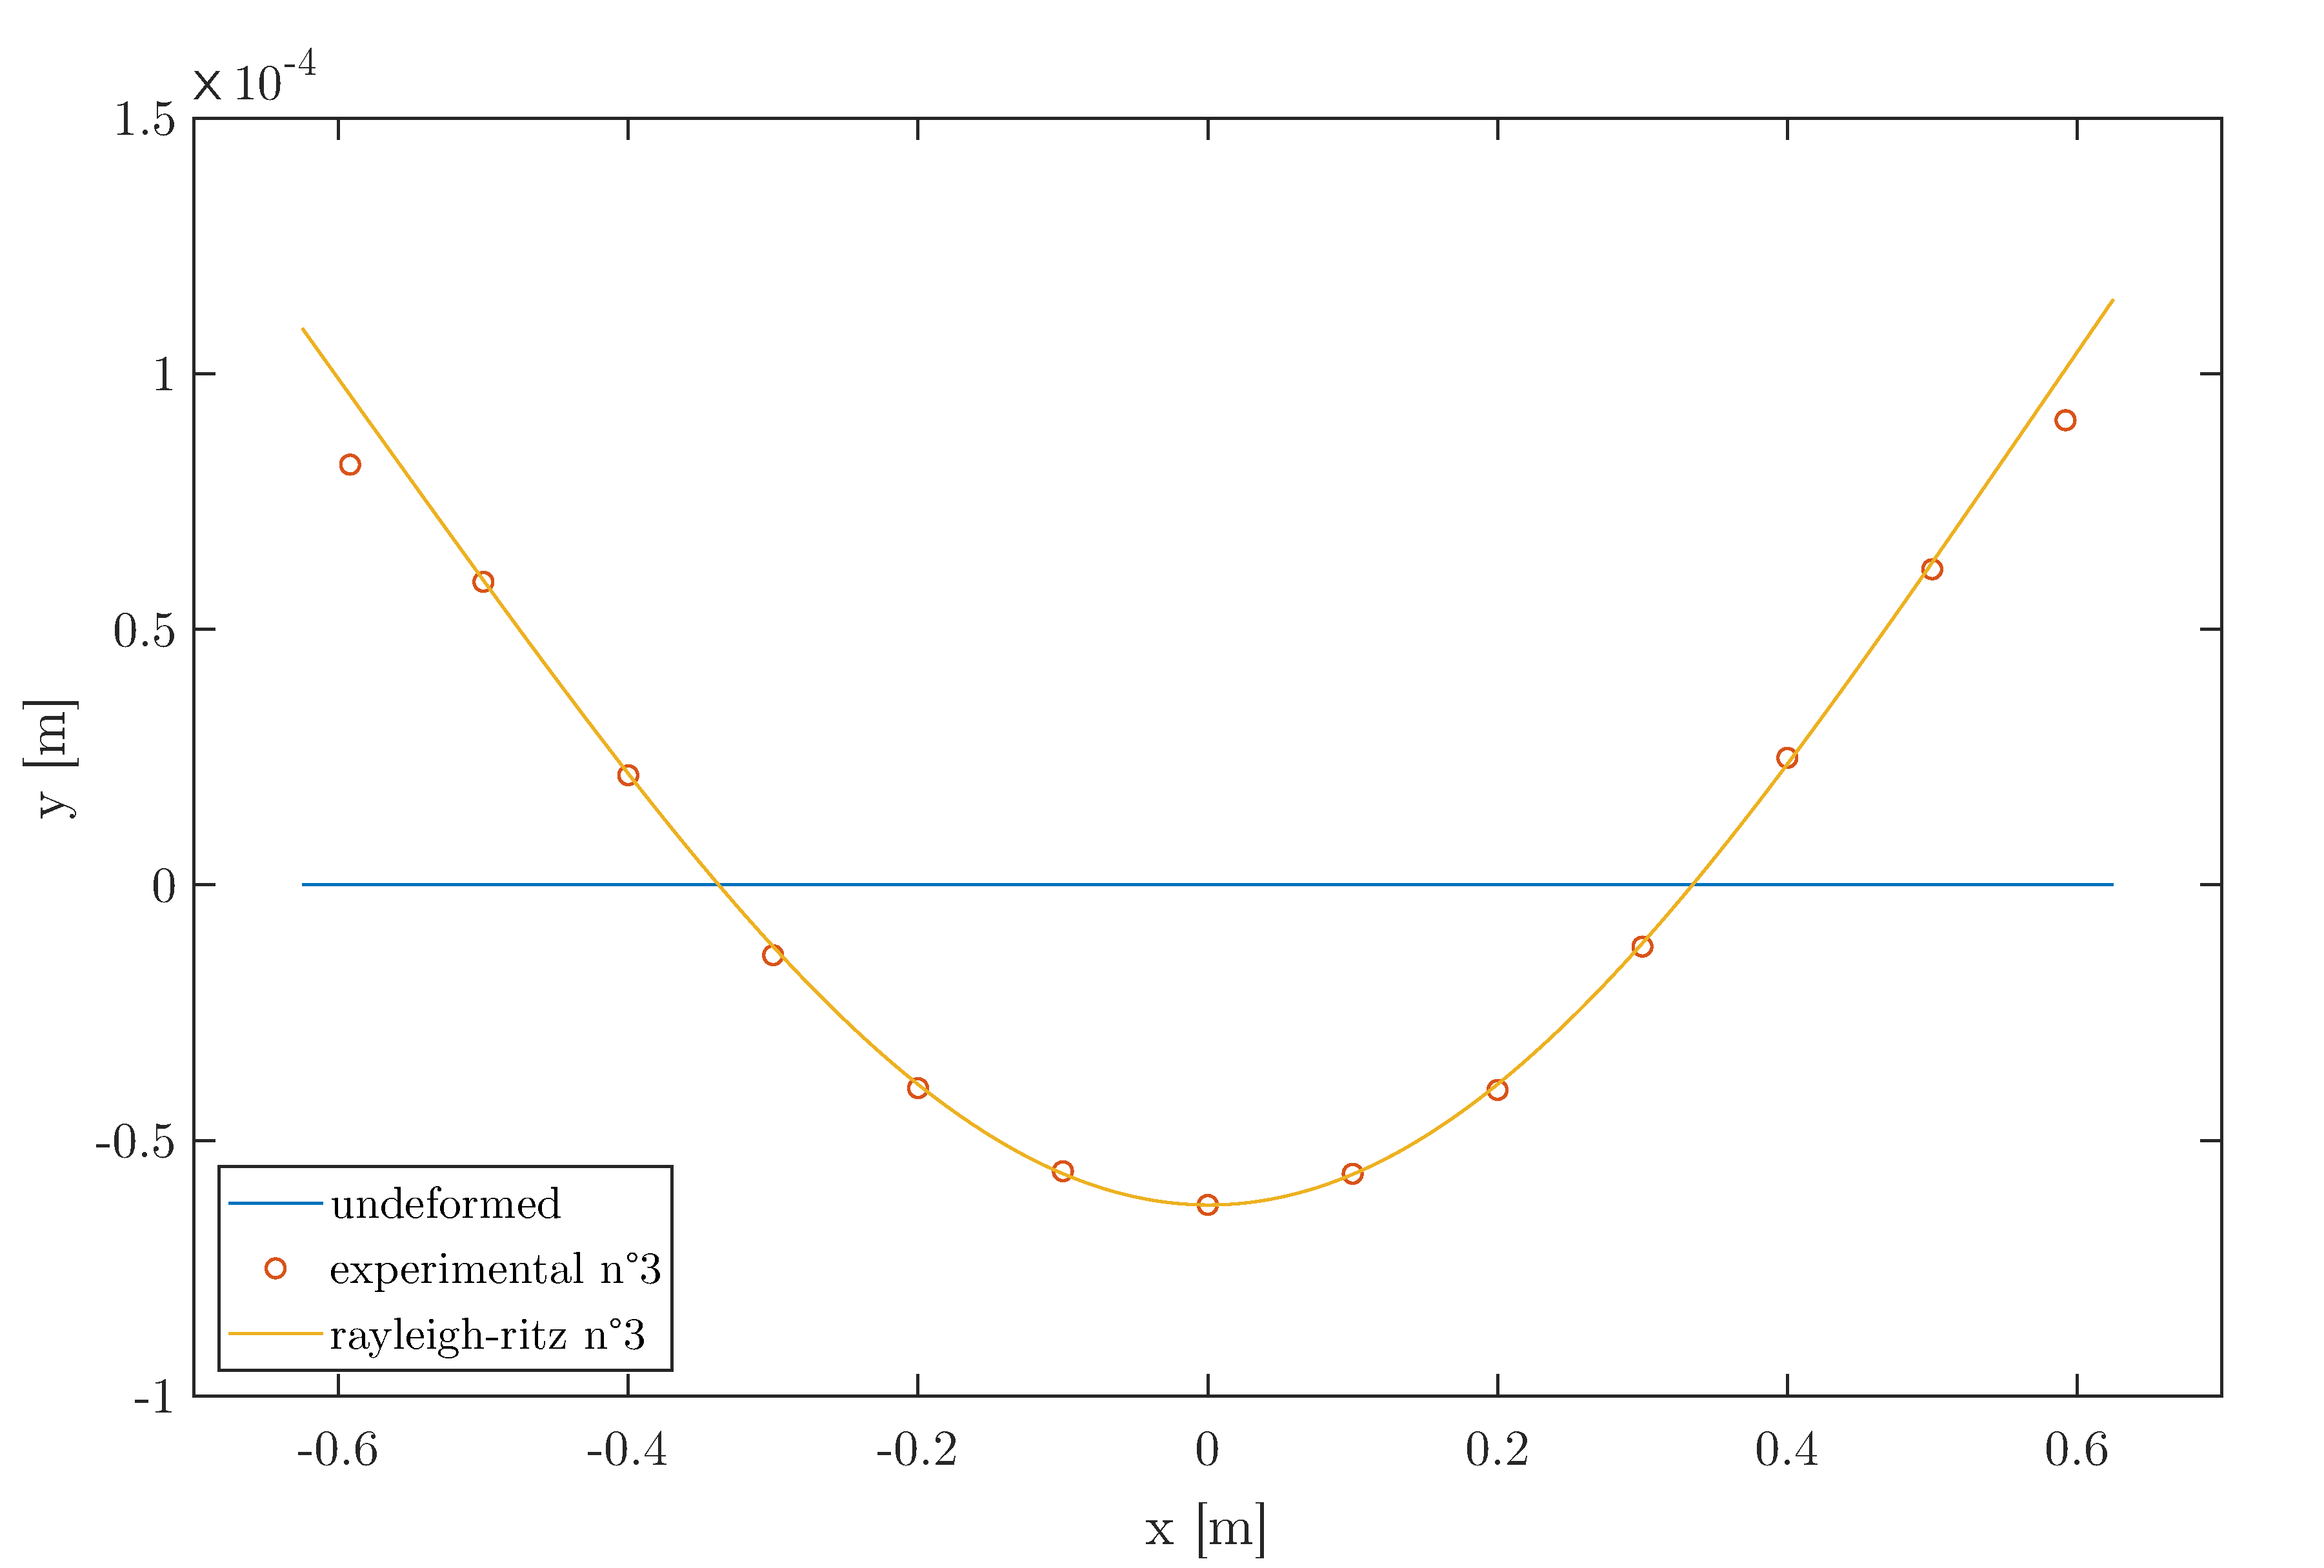
\includegraphics[width=1\textwidth]{resources/pdf/mode-shape3.pdf}
		\caption{Mode-shape \no 3}
		\label{figure:modeshape3}
	\end{figure}
	\begin{figure}[h]
		\centering
		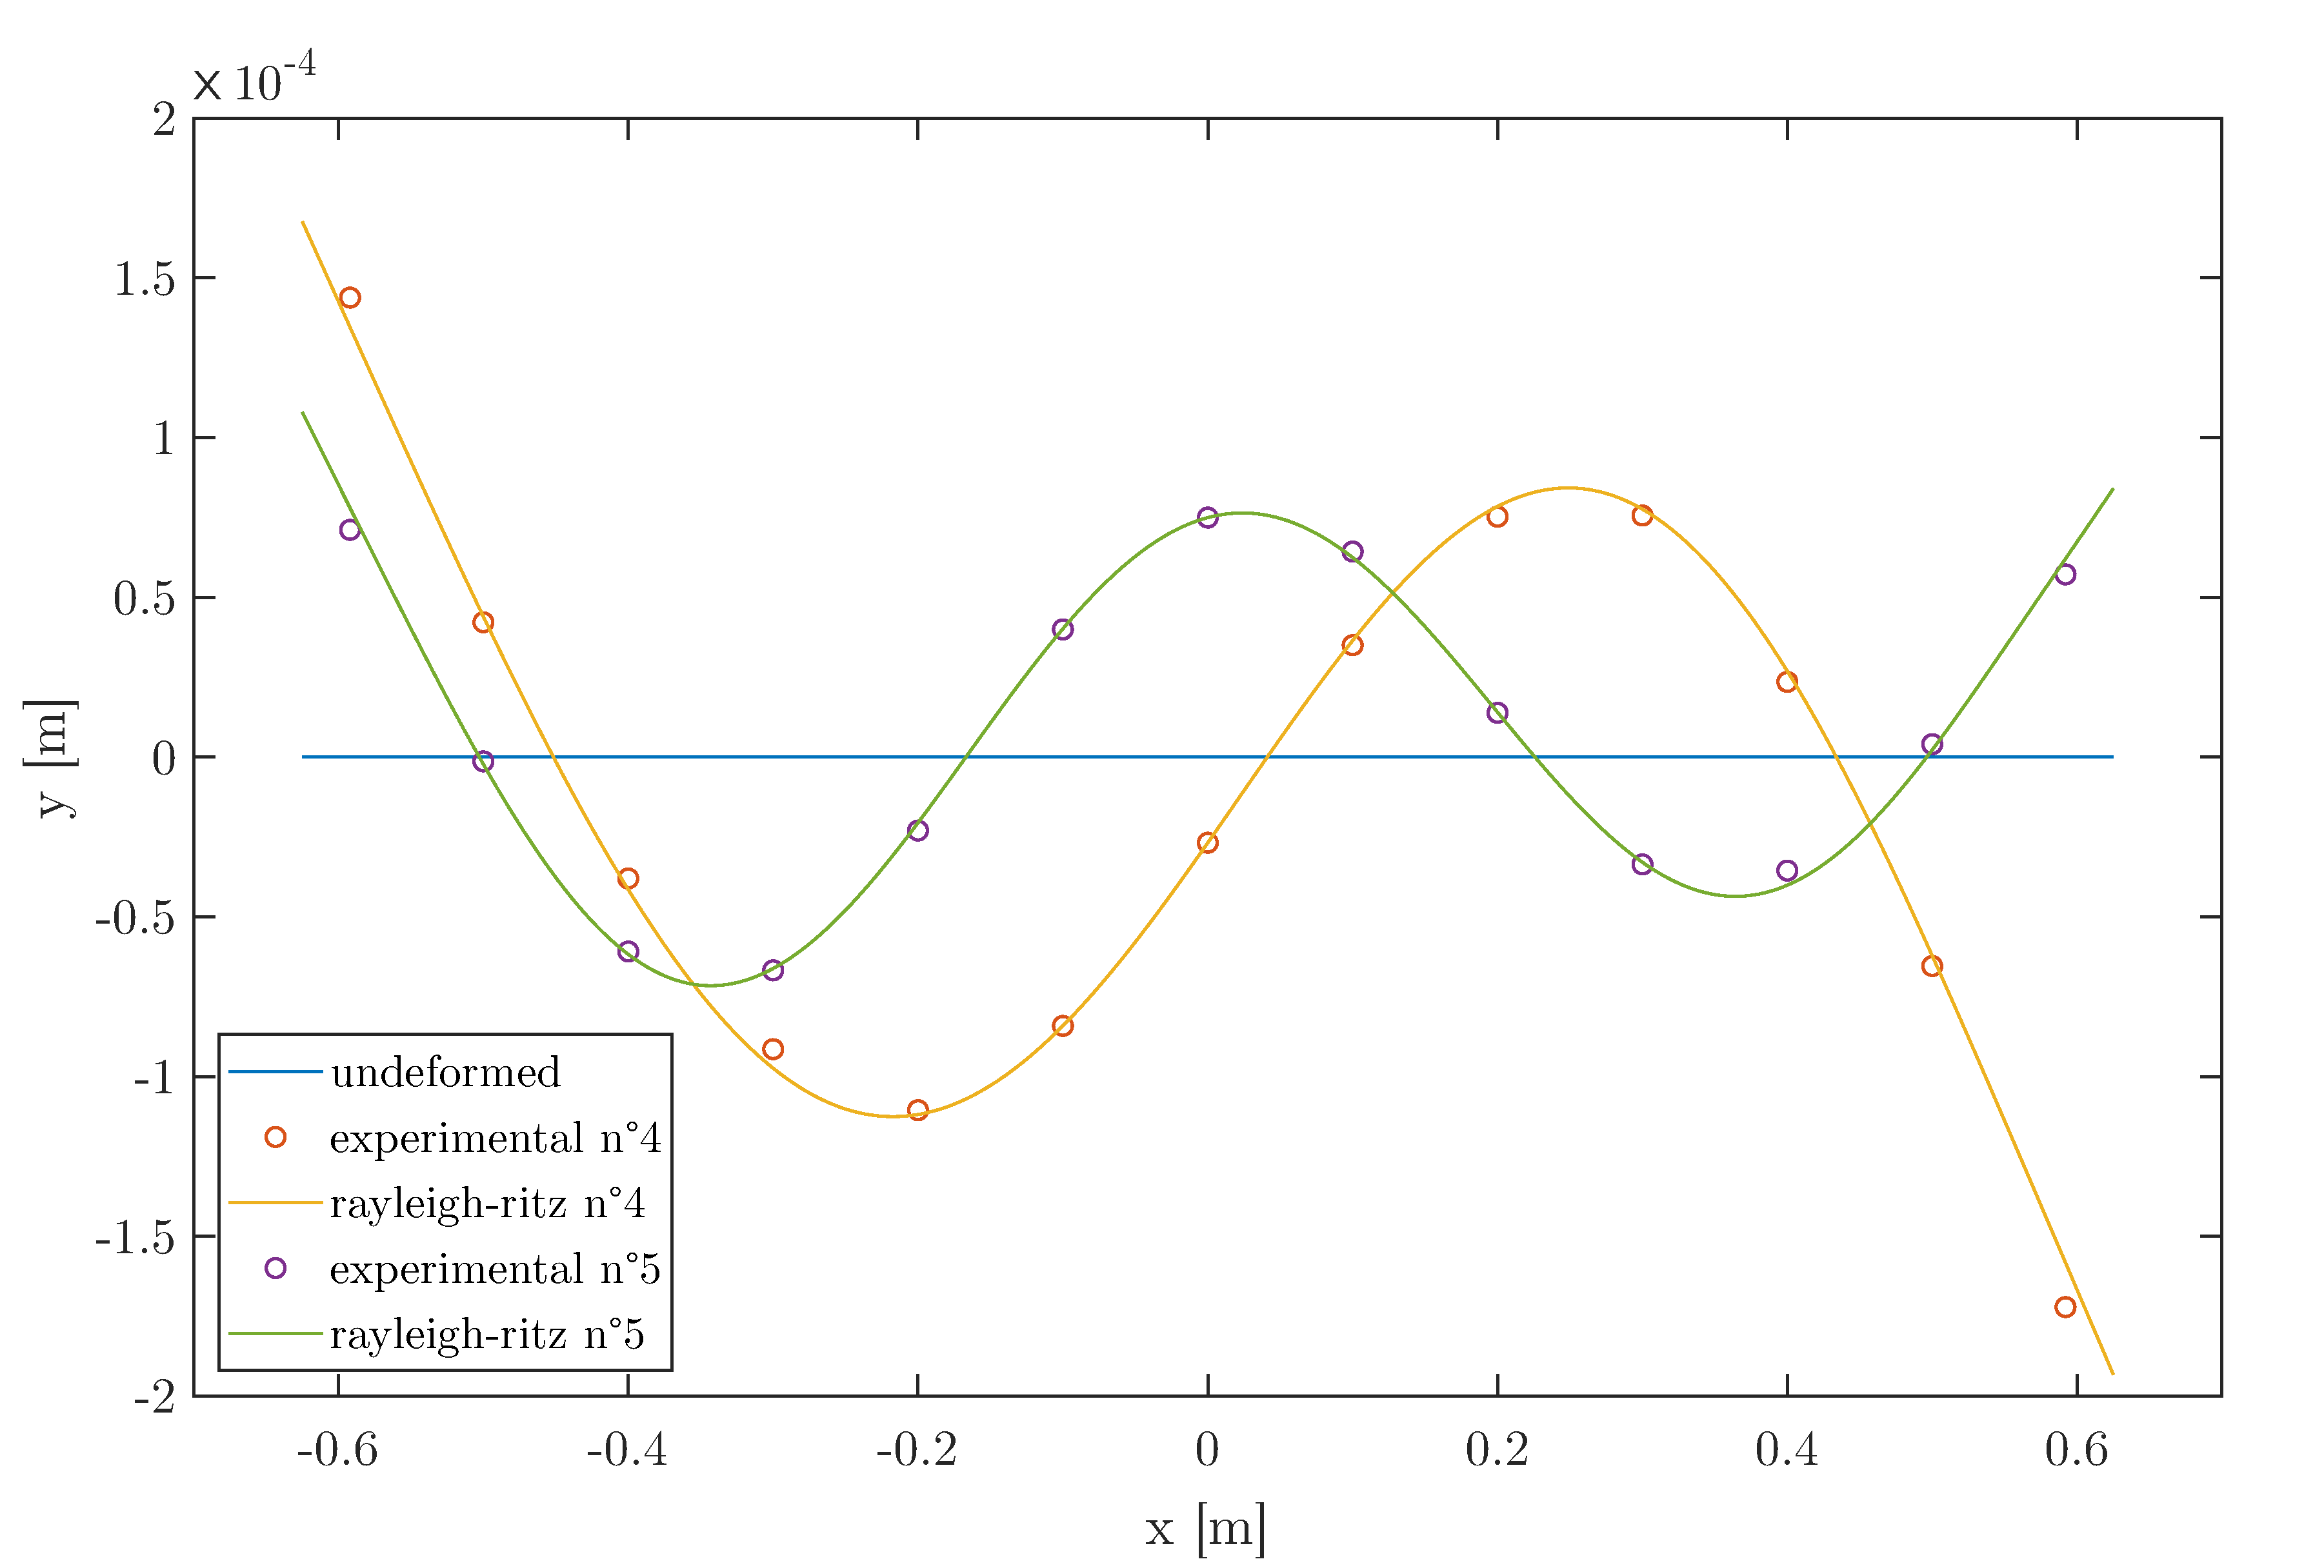
\includegraphics[width=1\textwidth]{resources/pdf/mode-shapes4and5.pdf}
		\caption{Mode-shapes \no 4 and 5}
		\label{figure:modeshape45}
	\end{figure}
	\clearpage
	\section*{Conclusions}
	In terms of frequency, both the 2 DOF model and the Rayleigh-Ritz method are close to the experimental measurements. The small relative errors ($\pm 1 \%$) could be due to inaccurate initial hypotheses. For example, we assumed in our analysis that the system was undamped which is actually impossible. Further, mechanical characteristics of the system such as masses, stiffnesses, dimensions, etc... could be imprecise as well. However, it seems that these approximations aren't entirely missguided given they produce good predictions. \par
	Nevertheless, we notice that the frequencies of the 2 DOF model are greater than Rayleigh-Ritz ones. But we know that Rayleigh-Ritz estimated frequencies are always greater than real ones. Therefore, the lowest frequencies are always the best. The 2 DOF model being equivalent to a Rayleigh-Ritz method with two degree of freedom, we can assume that the Rayleigh-Ritz results are better. \par
	In terms of modes, the Rayleigh-Ritz estimations are quite close to the measurements, as show figures \ref{figure:modeshape12}, \ref{figure:modeshape3} and \ref{figure:modeshape45}.
\end{document}
